\documentclass[tikz,border=5pt]{standalone}
\usetikzlibrary{shapes,arrows.meta,positioning}

% NOTE: don't use style name 'node' (reserved). Use 'blk'.
\tikzset{
  blk/.style={rectangle,rounded corners,draw=black,fill=blue!10,
              minimum width=2.8cm,minimum height=0.8cm,align=center},
  flowarrow/.style={-{Latex[length=3mm,width=2mm]},thick}
}

\begin{document}
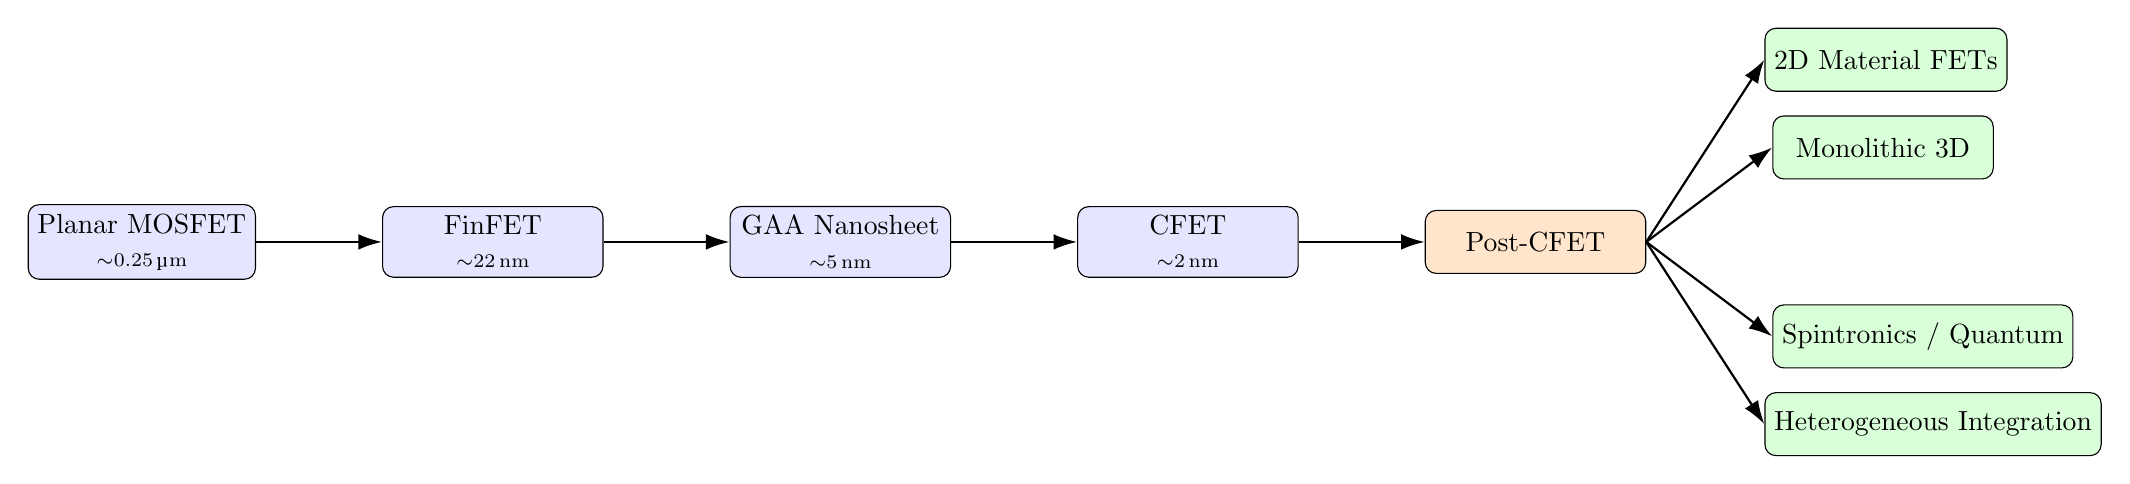
\begin{tikzpicture}[node distance=1.6cm]
  \node[blk] (planar) {Planar MOSFET \\ \scriptsize $\sim$0.25\,\textmu m};
  \node[blk, right=of planar] (finfet) {FinFET \\ \scriptsize $\sim$22\,nm};
  \node[blk, right=of finfet] (gaa) {GAA Nanosheet \\ \scriptsize $\sim$5\,nm};
  \node[blk, right=of gaa] (cfet) {CFET \\ \scriptsize $\sim$2\,nm};
  \node[blk, right=of cfet, fill=orange!20] (post) {Post-CFET};

  \draw[flowarrow] (planar) -- (finfet);
  \draw[flowarrow] (finfet) -- (gaa);
  \draw[flowarrow] (gaa) -- (cfet);
  \draw[flowarrow] (cfet) -- (post);

  % Branches
  \node[blk, above right=1.5cm and 1.5cm of post, fill=green!15] (f2d) {2D Material FETs};
  \node[blk, right=of post, yshift=1.2cm, fill=green!15] (m3d) {Monolithic 3D};
  \node[blk, right=of post, yshift=-1.2cm, fill=green!15] (spin) {Spintronics / Quantum};
  \node[blk, below right=1.5cm and 1.5cm of post, fill=green!15] (hetero) {Heterogeneous Integration};

  \draw[flowarrow] (post.east) -- (f2d.west);
  \draw[flowarrow] (post.east) -- (m3d.west);
  \draw[flowarrow] (post.east) -- (spin.west);
  \draw[flowarrow] (post.east) -- (hetero.west);
\end{tikzpicture}
\end{document}
